\setcounter{chapter}{6}
\chapter{Model Analysis}
\label{cha:model_analysis}
% \minitoc
% 
\section{Model parameter}
% 
In this thesis a universal sets of eigen-cubes shall be analysed/ created.
This sets of eigen-cubes should be usable to test hypothosis for the experimental setups \ac{LAP} and \ac{PM}.
\paragraph{fiber population orientation}
Furthermore it is necesarry, to get a resanable amount of possible fiber configurations.
Since the number of theoretical possible configurations is infinity, this has to be downsized.
Beginning with a single fiber population the main orientation $\modelOri$ can be anything on the orientationsphere.
However, since $f(\varphi,\alpha) = f(\varphi+\pi,-\alpha)$ only the orienatations of a halph spere are neceressy.
Furthermore the experimental setup lets no distingis bewten a fiber population with $\varphi = \varphi_0$ and $\varphi = \varphi_1$, if the initial optical elements are rotated be $\varphi_1-\varphi_0$ (expect camera pixel, will be neglected here).
Therefore it is not necesarry to create any single fiber population with a direction other than $varphi = 0$.
The inclination however has to be sample between the hole range $[0,90]\si{\degree}$. But since we can simple rotate a fiber population from $\varphi=0, \alpha=0$ to $\varphi=\varphi_{\text{rot}}, \alpha=\alpha_{\text{rot}}$, it is not necessary to build individual fiber configurations.
% 
\paragraph{two fiber bundle populations}
The same eigenschaften as above are true for the individual two fiber populations. This means, that only a differential angle between the two orientations, so called crossing angle $\modelOmega$, is needed as well as a density change between both populations \modelPsi in:
\begin{align}
    F_G = \modelPsi \cdot F_0 + (1-\modelPsi) \cdot F_1
\end{align}
% 
Since the direction of the first fiber bundle population can be again neglected, only the direction and inclination of the second fiber polulation rletaive to the first is importend. Therefore it was decided to build models with \modelOmega from ${0,10,...,90}$ and afterwords rotating the fiber orientations around the x axis (\cref{subfig:Test1})
% 
\paragraph{fiber population additional parameters}
density, dispersion, radii, change of radii, ...
% 
% 

\paragraph{rest}
% 
As described in \cref{chap5:ShapeControl} the choice of shape parameters \segLength and \segRadius are quite important. For a realistic fiber radius distribution of around \SI{0.5}{\micro\meter} the time for a \SI{60}{\micro\meter} usable cube (\SI{105}{\micro\meter} sphere) varies from several hours up to \SI{24}{\hour}.
% 
% 
\subsection{Setup}
% 

\begin{figure}[!t]
\centering
% \def\tikzwidth{0.5\textwidth}
\resizebox{0.5\textwidth}{!}{
\inputtikz{gfx/model/sphere_cube.tikz}}
\caption[]{A spherical volume with diameter $d$ is used as boundry for a fiber model, so that a cube of side length $1/1.5 \cdot d$ can be cut in any orientation inside the sphere.}
% \label{fig:}
\end{figure}
% 
\begin{figure}[!t]
\centering
\def\tikzwidth{0.5*\textwidth}
\subcaptionbox{fixed first fiber population; half rotation of second fiber population}[.49\textwidth]{
\inputtikz{gfx/model/sphere_models_.tikz}}\hfill
\subcaptionbox{\label{subfig:Test1}increasing inclination for first fiber population}[.49\textwidth]{
\inputtikz{gfx/model/sphere_models.tikz}}
\caption{two population model library}
\label{fig:twomodelpop}
\end{figure}
% 
\begin{table}[!b]
\sisetup{parse-numbers=false,open-bracket={\{}, close-bracket={\}}, list-final-separator={,},list-pair-separator={,}}%
\centering
\pgfplotstabletypeset[%
    thesisTableStyle,
    column type=lcl,
    columns/name/.style={string type},
    columns/variable/.style={string type},
    columns/values/.style={string type},
    every head row/.style={before row=\toprule,after row=\midrule},
    every last row/.style={after row=\bottomrule},
    col sep=&,
    row sep=\\,
    % string type,
]
{name & variable & values\\
mean fiber radius & $\fiberRadiusMean$ & $\SIlist{0.5;1;2;5;10}{\micro\meter}$\\
mean segment length factor & $\segLengthFactor$ & $\SIlist{1;2;4;8}{\micro\meter}$\\
min segment bending radii factor & $\segRadiusFactor$ & $\SIlist{1;2;4;8}{\micro\meter}$\\
fiber bundle distribution value & $\modelPsi$ & $\SIlist{0.1;0.2;...;1.0}{}$ \\
fiber bundle crossing angle & $\modelOmega$ & $\SIlist{0;10;...;90}{\degree}$\\
}
\caption{parameter\_statistic setup and \textcolor{violet}{variables}.}
% \label{}
\end{table}
% 
\begin{table}[!b]
\centering
\sisetup{open-bracket={\{}, close-bracket={\}}, list-final-separator={,},list-pair-separator={,}}%
\pgfplotstabletypeset[%
    thesisTableStyle,
    column type=l,
    columns/variable/.style={string type},
    columns/value/.style={string type},
    every head row/.style={before row=\toprule,after row=\midrule},
    every last row/.style={after row=\bottomrule},
    col sep=&,
    row sep=\\,
]
{variable & value\\
pre model diameter & $d = \SI{105}{\micro\meter}$\\
mean fiber radius & $\textcolor{violet}{\fiberRadiusMean} = \SIlist{0.5;1;2;5;10}{\micro\meter}$\\
fiber radius distribution & $\fiberRadiusSig = \SI{0.1}{}$, $\fiberRadiusMu = \SI{0}{\micro\meter}$\\
seed.distance & $2 \cdot \textcolor{violet}{\fiberRadiusMean}$\\
seed.size & $2 \cdot \mathit{volume}$\\
bundle distribution & $\textcolor{violet}{\modelPsi}$\\
bundle crossing & $\textcolor{violet}{\modelOmega}$\\
solver.obj\_mean\_length & $\fiberRadiusMean \cdot \textcolor{violet}{\segLengthFactor}$\\
solver.obj\_min\_radius & $\fiberRadiusMean \cdot \textcolor{violet}{\segRadiusFactor}$\\
solver.max\_steps & $\SI{100000}{}$\\
max runtime & $\SI{24}{\hour}$\\
}
\caption{parameter\_statistic setup and \textcolor{violet}{variables}.}
% \label{}
\end{table}
% 
% 
\begin{figure}[!t]
\centering
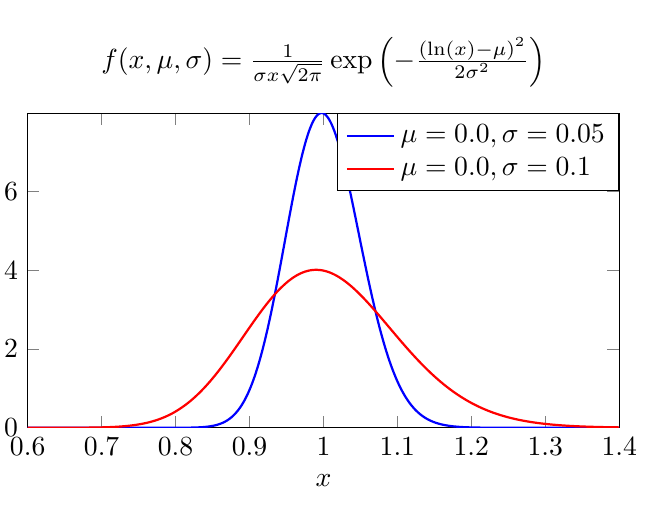
\begin{tikzpicture}[scale=1, trim axis left, trim axis right]
\begin{axis}[height=0.46\textwidth, width=0.75\textwidth,enlargelimits=false, xlabel={$x$}, ylabel={$f(x,\mu,\sigma)$}, title=${f(x,\mu,\sigma)=\frac{1}{\sigma x \sqrt{2\pi}}\exp\left(-\frac{(\ln(x)-\mu)^2}{2 \sigma^2}\right)}$,
legend style={at={(1,1)},anchor=north east},
legend cell align={left},
]
\pgfmathsetmacro{\muValue}{0}
\pgfmathsetmacro{\sigmaValue}{0.05}
\addplot[blue,thick,domain=0.6:1.4, samples=1000]{1/(\sigmaValue*x*sqrt(2*pi))*exp(-(ln(x)-\muValue)^2/(2*\sigmaValue^2))}; \addlegendentry{$\mu=0.0,\sigma=0.05$}
\pgfmathsetmacro{\muValue}{0}
\pgfmathsetmacro{\sigmaValue}{0.1}
\addplot[red,thick,domain=0.6:1.4, samples=1000]{1/(\sigmaValue*x*sqrt(2*pi))*exp(-(ln(x)-\muValue)^2/(2*\sigmaValue^2))}; \addlegendentry{$\mu=0.0,\sigma=0.1$}
\end{axis}
\end{tikzpicture}
\caption[]{\todo{check values in literatur}}
% \label{fig:}
\end{figure}
% 
\subsection{Results}
% 
\todo{STRANGE behaviour in parameter\_statistic for smaller radii. probably because of rnd seeds}
% 
\begin{figure}[!t]
\centering
\includegraphics[width=\textwidth, page=1]{dev/gfx/2/parameter_statistic_box_plot.pdf}
\caption{Model (\fiberRadius) characteristic for different parameters}
% \label{fig:}
\end{figure}
% 
\begin{figure}[!t]
\centering
\includegraphics[width=\textwidth, page=2]{dev/gfx/2/parameter_statistic_box_plot.pdf}
\caption{Model characteristic for different parameters}
% \label{fig:}
\end{figure}

\begin{figure}[!t]
\centering
\includegraphics[width=\textwidth]{dev/gfx/2/parameter_statistic_time_evolve.pdf}
\caption[Time development of the model generation process.]{Time development of the model generation process.}
% \label{fig:}
\end{figure}
% 
\subsection{Discussion}
% 
The goal is to choice a set of parameters, which allow a) fast, b) collision free and c)a high volume fraction for densely fibers. 
%  
\subsubsection{timeing}
% 
\paragraph{is overlap important?}
% 
analog analysis like voxelsize -> simulation?
% 
\section{CPU Acceleration}
% 
As described in \dummy \openmp is used for acceleration.
This means no usage of multiple computer nodes is currently available.
Since the Code traverses an octree, This would not be feasable.
Also more then 8 cores \dummy.
% 
\subsection{Setup}
% 
\subsection{Results}
% 
\subsection{Discussion}
% 
\begin{figure}[!t]
\centering
\includegraphics[]{dev/gfx/4/model_solver_cubes.pdf}
\caption{}
% \label{fig:}
\end{figure}
% 
\section{Building models for simulation}
% 
\subsection{Setup}
% 
\subsection{Results}
% 
\begin{figure}[!t]
\centering
% \resizebox{1.0\textwidth}{!}{
\includegraphics[width=\textwidth, page=1]{dev/gfx/2/cube_2pop_orientation_hist.pdf}
% }
\caption{}
% \label{fig:}
\end{figure}
% 
\subsection{Discussion}

